\chapter{Navržená hra - Asteroidy}

\section{Herní logika}
Jedná se o hru dvou hráčů. 
Každý z hráčů ovládá svou vesmírnou loď.
Prostředí hry má představovat vesmírný prostor, je to ale prostor zjednodušený, proto zde neplatí gravitační ani odporové síly.
To má tedy za následek, že když se vesmírná loď rozletí v nějakém směru, tak v tomto směru letí i nadále i bez dalšího akcelerování.
\par
\label{HraniceProsotru}
Vesmírný prostor je v této hře nekonečný a dalo by se říct jistým způsobem cyklický, pokud vesmírná loď proletí dolní hranicí herního prostoru, tak nezmizí, ani nenabourá, ale objeví se na stejné pozici jen na horní hranici a obráceně. Analogicky to platí i s bočními hranicemi.
Vesmírné lodě sebou mohou proletět a nedojde ke srážce.
Nejsou zde žádné statické překážky, kterým by bylo třeba se vyhnout. Co se ale může srazit s vesmírnou lodí jsou asteroidy.    
\par
Asteroidy vznikají v průběhu hry na náhodných místech a letí náhodným směrem. Nové asteroidy se generují častěji, čím déle hra trvá.
V boji s asteroidy má hráč v zásadě dvě možnosti. Buď se může pokusit danému asteroidu vyhnout, tím že s lodí pohne mimo trajektorii asteroidu, anebo může asteroid sestřelit.
Každý hráč má omezený počet životů a každá srážka lodě s asteroidem ubere hráči část jeho životů.
\par
Hráč má k dispozici dva typy střel, obyčejnou a rozdvojovací. Vystřelená střela má značně vyšší rychlost než vesmírné lodě i než kolem letící asteroidy.
Střely nejsou určeny k přímému zasažení lodě protihráče, vesmírné lodě jsou k nepřátelké střele imunní.
Střely jsou určený k sestřelování letících asteroidů. Asteroidy mohou mít tři velikosti. Náhodně vytvořený asteroid je vždy největší. Každým rozstřelením daného asteroidu vznikají asteroidy o stupeň menší velikosti.
Nově vytvořené asteroidy vznikají na místě původního asteroidu. Asteroid se může rozstřelit různými způsoby. Zde záleží na tom, jakou střelou byl asteroid setřelen. 
\par
V případě střely obyčejné vznikne namísto původního asteroidu jeden menší, který letí stejným směrem jako střela, která ho zasáhla.
V případě střely rozdvojovací se původní asteroid rozstřelí na dva menší, kde každý z nich je oproti směru střely vychýlen o 15\textdegree po a proti směru hodinnových ručiček.
Pokud je zasažen asteroid nejmenší velikosti, tak již žádné další asteroidy nevznikají. 
Rychlost asteroidů je nepřímo závislá na jejich velikosti, čím je asteroid menší, tim vyšší rychlost má.
\par
Asteroidy vzniklé rozstřelením se stávají projektily daného hráče. Hráč nemůže být zasažen asteroidem, který sám vytvořil

\begin{figure}[p]

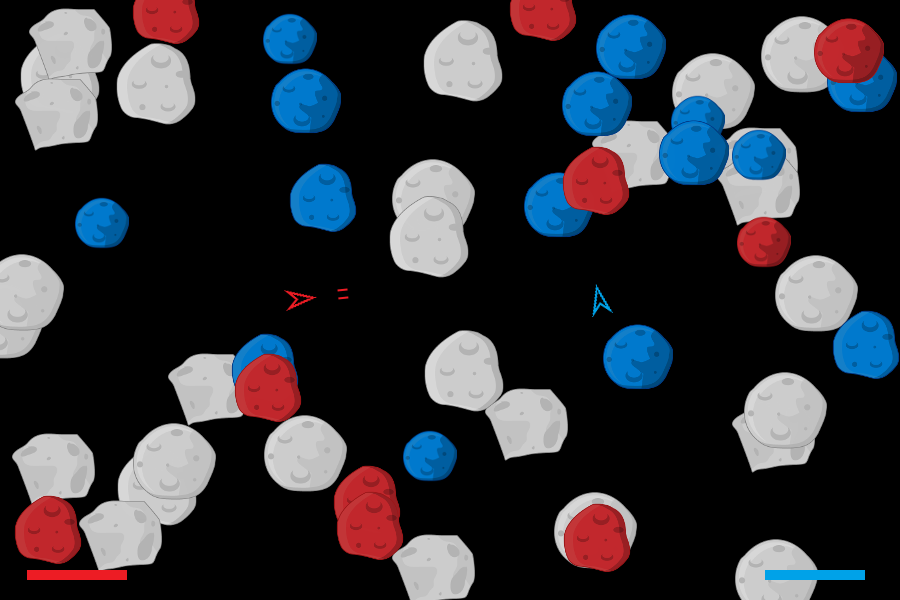
\includegraphics[width=150mm, height=100mm]{./Obrazky/UkazkaHry.png}
\caption{Screenshot ze hry}
\label{obr01:}
\end{figure}


\section{Cíl hry}
Během hry vzniká postupně více a více asteroidů, čímž je postupně stále obtížnější se všem asteroidům vyhnout, nebo je sestřelit.
Hráč nemůže zranit nepřítele střelou přímo, může se ale snažit rozstřelit nějaký z kolem letících asteroidů tak, aby pomocí nově vzniklých asteroidů trefil nepřítele.
Cílem hráče je ovládat svou loď takovým způsobem, aby vydržel ve hře déle. Hra končí a hráč vítězí, když nepříteli nezbydou žádné další životy.

